%! TeX root: ../thesis_a4.tex

\chapter{Synthetic Room Impulse Responses for Monaural Speech Enhancement}
\chaptermark{Synthetic RIRs for SE}
\label{ch04_mbrirs}

The previous chapter highlighted, for the specific case of \acrshortpl{HA}, the importance of the data a model is trained and evaluated on. This chapter carries the same idea to general-purpose \acrshort{SE}, again within the context of the GuestXR project, and again keeping the focus on one particular ingredient of its training data: the \acrfullpl{RIR} used to simulate reverberation. As we saw in Chapter~\ref{ch03_hearing}, while \acrshortpl{HA} are beginning to adopt \acrshortpl{DNN}, they do so under tight latency and power constraints. For normal-hearing listeners in settings such as videoconferencing, where those constraints are far looser, \acrshort{DNN}-based \acrshort{SE} has instead thrived, to the point that neural noise suppression now runs in virtually every videoconferencing application. This success has been driven in no small part by ever larger and more diverse training sets, such as those of the \acrfull{DNS} challenges \citep{dns5}.

Scaling the amount and variety of data has produced models that generalise better and narrow the cross-dataset performance gaps discussed in
Chapter~\ref{ch02_sota} \citep{richter2023speech, kadiouglu2020empirical}, and
extending speech and noise material to a $48\,\text{kHz}$ sampling rate has
improved results further \citep{schroter2023deepfilternet3, zhang2023toward,
zhang2024urgent}. Again, the standard recipe for injecting acoustic diversity is to convolve clean speech with a \acrshort{RIR}, placing it in a variety of
simulated rooms. The scaling and development of \acrshort{RIR} datasets themselves, however, have not kept pace. As noted in the
dataset review of Chapter~\ref{ch02_sota}, most \acrshort{SOTA} systems still train on the \acrshortpl{RIR} of the early \acrshort{DNS} challenges \citep{ko2017study}: shoebox rooms rendered with the \acrfull{ISM}
(Section~\ref{sec:bg_rir_ism}), at a $16\,\text{kHz}$ sampling rate, and with a
\emph{single} absorption coefficient shared across the whole frequency
spectrum. In fact, the \acrshortpl{RIR} of the \acrshort{DNS} challenge were originally assembled for \acrshort{ASR} rather
than enhancement. 

Increasing the realism of the \acrshortpl{RIR}
has already been shown to help related tasks such as \acrshort{ASR} for
augmented-reality glasses \citep{arakawa2024quantifying} or keyword spotting
\citep{bezzam2020study}, even when applied only as a post-processing
augmentation \citep{ratnarajah2021ts}, so the same should hold for monaural general-purpose \acrshort{SE}. This raises the question of \emph{which} properties of a synthetic \acrshort{RIR} actually matter for \acrshort{SE} generalisation to real acoustics (\textbf{RO3}).

Other recent efforts point in the same direction: the URGENT challenge \citep{zhang2024urgent} pushes \acrshort{SE}
towards \emph{universality} and \emph{robustness}, bringing together
denoising, dereverberation, declipping, bandwidth extension and other
distortions in a single task, spanning a wide range of sampling rates, and, tightly related to our approach, evaluating on real recorded \acrshortpl{RIR}
rather than only synthetic ones, which highlights the importance of ecological validity. However, the URGENT challenge still
trains on the ten-year-old \acrshortpl{RIR} from \acrshort{DNS}5. In a similar line of work, generative augmentation of existing
\acrshortpl{RIR} has been explored in \citet{GenDA2025_RoomAcoustics}.

As we introduced in Chapter~\ref{ch02_sota}, some recent \acrshort{RIR} datasets use path tracing over 3D meshes of realistic geometries, mainly for tasks beyond
monaural \acrshort{SE} such as audio-visual navigation
\citep{kelley2024rir, tang2022gwa}. Its best-known instance is the SoundSpaces
dataset \citep{chen2022soundspaces}, which provides a dense grid of receiver
positions within each room. However, it
spans comparatively few distinct rooms, and how models trained on its \acrshortpl{RIR} perform on the \acrshort{SE} task remains unclear. GWA~\citep{tang2022gwa} is likewise mesh-based and does report
dereverberation and separation experiments, but only uses intrusive metrics on a very limited number of rooms. Whether such geometrically realistic
yet scarce mesh-based \acrshortpl{RIR} are preferable to abundant but simpler
shoebox ones is still not well understood (\textbf{RO4}).

To tackle both \textbf{RO3} and \textbf{RO4}, 
we evaluate six models trained on the same speech and noise datasets but on six different \acrshort{RIR} datasets (two baselines, three of our own making and one set of SoundSpaces), with the intention of answering whether models benefit from using RIRs with frequency dependent (multiband) absorption coefficients, whether modeling the receiver directivity or the source directivity helps to generalize in monaural models, and whether mesh-based modeling might be helpful or more suitable than \acrshort{ISM}~\citep{bezzam2020study}. To this end, we propose an evaluation of the following RIR datasets, which are summarized in Table \ref{tab:ch4_datasets}:

\begin{itemize}
    \item  \textbf{DNS5}: the \acrfull{SOTA} baseline from \citet{ko2017study}.
    \item \textbf{SB}: recreation of the \acrshort{DNS}5 at 48\,kHz sampling rate using \textbf{s}ingle-\textbf{b}and absorption coefficients on the shoebox room material.
    \item \textbf{MB}: same as SB but using \textbf{m}ulti-\textbf{b}and absorption coefficients instead.
    \item \textbf{REC+MB}: same as MB but adding \textbf{rec}eiver directivity by using \acrshortpl{HRTF} at the rendering stage.
    \item \textbf{SRC+REC+MB}: adding \textbf{s}ou\textbf{rc}e directivity by modelling average human speech directivity in the \acrshort{ISM}.
    \item \textbf{SSPA}: we use mesh-based RIRs from \textbf{S}ound\textbf{Spaces} instead.
\end{itemize}



Keeping the speech, the noise and the room geometries fixed,
we train one \acrshort{SE} model on each and evaluate it on \emph{real} \acrshortpl{RIR}, both objectively and through a listening test. We find that
frequency-dependent absorption is always a beneficial feature, and we
release the resulting multiband \acrshort{RIR} dataset, \emph{MB-RIRs}, as well as the multiband with source and receiver directivities, \emph{SRC+REC+MB-RIRs}, as freely available research
materials\footnote{\url{https://doi.org/10.5281/zenodo.15773093}}.


\begin{table}[htbp]
\centering
\footnotesize
\renewcommand{\arraystretch}{1.25}
\caption{The six synthetic \acrshort{RIR} datasets under comparison and their sampling rate, absorption coefficients, receiver directivity, source directivity and rendering method. The first two are baselines, the next three are our own making, and the last one is a pre-computed mesh-based.}
\label{tab:ch4_datasets}
\begin{tabular}{@{}lccccc@{}}
\toprule
 & $f_s$ & Absorption coeff. & Receiver Dir. & Source Dir. & Renderer \\
\midrule
DNS5        & 16\,kHz & single & \xmark & \xmark & \acrshort{ISM}  \\
SB          & 48\,kHz & single & \xmark & \xmark & \acrshort{ISM}  \\
MB          & 48\,kHz & multi  & \xmark & \xmark & \acrshort{ISM}  \\
REC+MB      & 48\,kHz & multi  & \cmark & \xmark & \acrshort{ISM}  \\
SRC+REC+MB  & 48\,kHz & multi  & \cmark & \cmark & \acrshort{ISM}  \\
SSPA        & 48\,kHz & multi  & \cmark & \xmark & mesh-based \\
\bottomrule
\end{tabular}
\end{table}

\section{Training datasets}
\label{sec:mbrirs_datasets}

It is important to stress that the six models evaluated in this chapter differ \emph{only} in the \acrshortpl{RIR} used to reverberate their training data; the clean speech and the noise are identical across all of them, so that any difference in performance can be attributed to the room acoustics alone. For both we use the entire \acrshort{DNS}5 corpus \citep{dns5}, a large and deliberately heterogeneous collection: emotional speech, English audiobook readings in a range of accents, singing voice from VocalSet, multilingual speech (French,Spanish, Italian, Russian and German from M-AILABS, German from Wikipedia, and the Spanish OpenSLR sets SLR73, SLR61, SLR39, SLR75, SLR74 and SLR71), together with noise from FreeSound and AudioSet.
In total this amounts to $583$k speech utterances ($1{.}315$ hours) and $63$k
noise samples ($177$ hours). We split both into $70\%$ for training and the
remaining $30\%$ divided equally between validation and test, avoiding
speaker contamination across splits wherever the metadata allowed it. The rest
of this section describes the six \acrshort{RIR} sets built on top of this
shared material.

\subsection{Baseline RIRs (DNS5)}
\label{ssec:mbrirs_dns5}


Our baseline is the \acrshort{RIR} set of the \acrshort{DNS}5 challenge itself
\citep{ko2017study}. These
\acrshortpl{RIR} come from two companion collections released with that work:
the roughly $60$k \emph{synthetic} shoebox responses of OpenSLR26, rendered
with the \acrfull{ISM} (Section~\ref{sec:bg_rir_ism}) for small, medium and
large rooms, and the $325$ \emph{real} measured responses of OpenSLR28,
gathered from the RWCP, REVERB and Aachen (AIR) databases and spanning
everything from small meeting rooms to large auditoria. Both were originally
distributed at $16\,\text{kHz}$; we take $60$k of them, distribute the small,
medium and large rooms into the same $70\%/15\%/15\%$ training, validation and
test splits used throughout, and upsample everything to $48\,\text{kHz}$ for
compatibility with the other sets. This baseline carries the two limitations
that motivate the rest of the chapter: it is effectively band-limited by its
original $16\,\text{kHz}$ rendering, and its shoebox responses use a
\emph{single} absorption coefficient across the whole spectrum.

\subsection{Single-band absorption coefficients RIRs (SB)}
\label{ssec:mbrirs_sb}

The \acrshort{DNS}5 baseline conflates two limitations at once: it is
band-limited (rendered at $16\,\text{kHz}$) and single-band in absorption. To
isolate the first, and to obtain a controlled counterpart to our own datasets,
we re-create an approximation of it at $48\,\text{kHz}$ while keeping the single
absorption coefficient. We generate $60$k shoebox \acrshortpl{RIR} with the
\acrshort{MASP} library \citep{perez2020parametric, politis2016microphone}, the
same \acrshort{ISM} simulator used for the hearing-aid scenes of
Chapter~\ref{ch03_hearing}. Comparing the resulting \textbf{SB} set with
\acrshort{DNS}5 therefore isolates the effect of sampling rate alone.

The random room configuration is summarised in Table~\ref{tab:mbrirs_rooms}.
Crucially, it is drawn \emph{once} and reused \emph{identically} across all
four of our \acrshort{ISM}-based datasets (SB, MB, REC+MB and SRC+REC+MB): the
same rooms, the same receiver and source placements, and the same reverberation
times. The four sets thus differ only in the acoustic feature under study ---
the number of absorption bands and the receiver and source directivity --- so
that any change in performance can be attributed to that feature alone rather
than to a different sampling of geometries. Only the pre-computed SoundSpaces
set (SSPA) uses its own rooms, as it cannot share this configuration.

Within each room, the dimensions $\boldsymbol{r}$ are drawn from uniform
distributions, with the depth $r_y$ made relative to the width $r_x$ to avoid
implausible, corridor-like geometries. The receiver $\boldsymbol{rec}$ is placed
at random, away from the walls, and the source $\boldsymbol{src}$ around it,
between $0.5$ and $3\,\text{m}$ away and roughly in front. The single absorption
coefficient of the six walls then follows from Sabine's formula
(Section~\ref{sec:bg_rir_ism}) given $\boldsymbol{r}$ and a target reverberation
time $T_{60}$. For consistency with the multiband case of
Section~\ref{ssec:mbrirs_mb} --- where $\boldsymbol{T_{60}}$ is a vector, one
value per frequency band --- the scalar $T_{60}$ used here is the mean of that
vector, which turns out to be well approximated by a normal distribution.


\begin{table}[htbp]
\centering
\footnotesize
\caption{Random room configuration shared by the \acrshort{ISM}-based datasets
(SB, MB, REC+MB, SRC+REC+MB), sampled from the uniform distribution
$\mathcal{U}$ (and, for the reverberation time, the Gamma and normal
distributions). Dimensions, positions and distances are in metres and angles
in degrees; bold symbols are vectors.}
\label{tab:mbrirs_rooms}
\begin{tabular}{@{}lll@{}}
\toprule
Variable & Description & Distribution \\
\midrule
$r_x$ & room width  & $\mathcal{U}(3, 30)$ \\
$r_y$ & room depth  & $r_x \cdot \mathcal{U}(0.5, 1)$ \\
$r_z$ & room height & $\mathcal{U}(2.5, 5)$ \\[2pt]
$rec_x$ & receiver position along $x$ & $\mathcal{U}(0.35\,r_x,\, 0.65\,r_x)$ \\
$rec_y$ & receiver position along $y$ & $\mathcal{U}(0.35\,r_y,\, 0.65\,r_y)$ \\
$rec_z$ & receiver height             & $\mathcal{U}(1, 2)$ \\[2pt]
$rec_\phi$   & receiver azimuth   & $\mathcal{U}(-45, 45)$ \\
$rec_\theta$ & receiver elevation & $\mathcal{U}(-10, 10)$ \\[2pt]
$\lVert \boldsymbol{rec} - \boldsymbol{src} \rVert$ & receiver--source distance & $\mathcal{U}(0.5, 3)$ \\
$\angle\, \boldsymbol{rec}, \boldsymbol{src}$       & receiver--source angle    & $\mathcal{U}(-45, 45)$ \\[2pt]
$\boldsymbol{T_{60}}$ & per-band reverberation time & $\mathrm{Gamma}(\boldsymbol{\alpha}, \boldsymbol{\beta})$ \\
$T_{60}$              & broadband reverberation time & $\tfrac{1}{N}\sum_{n} \boldsymbol{T_{60}} \approx \mathcal{N}(0.4,\, 0.014)$ \\
\bottomrule
\end{tabular}
\end{table}


\subsection{Multiband absorption coefficients RIRs (MB)}
\label{ssec:mbrirs_mb}

The first and central of our three \acrshort{ISM} strategies is to replace the
single broadband absorption coefficient of SB with a
\emph{frequency-dependent} one, so that each wall absorbs differently across
the spectrum, as real materials do. 

\begin{figure}[htpb]
  \centering
  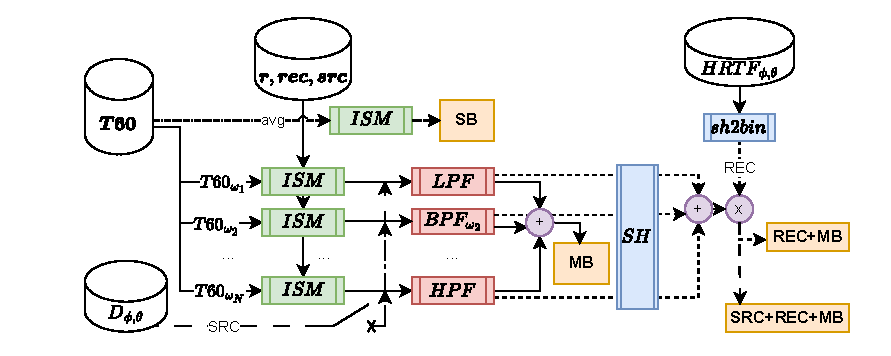
\includegraphics[width=\columnwidth]{ch04_mbrirs/figures/pipeline.pdf}
  \caption{The \acrshort{RIR} generation pipeline. All \acrshort{ISM}-based
  datasets share the same geometric configurations. The dotted line is the
  single-band path (SB); the continuous line adds the per-band absorption and
  filterbank of MB; the short-dashed line adds receiver directivity (REC+MB)
  and the long-dashed line the source directivity (SRC+REC+MB).}
  \label{fig:mbrirs_pipeline}
\end{figure}

Concretely, instead of a single scalar $T_{60}$ we now sample a vector
$\boldsymbol{T_{60}}$ of reverberation times, one per frequency band, over the
six octave bands $\boldsymbol{\omega} = \{125, 250, 500, 1\text{k}, 2\text{k},
4\text{k}\}\,\text{Hz}$, as illustrated in Figure~\ref{fig:mbrirs_pipeline}.To keep these vectors realistic rather than arbitrary, we fit their
distribution to measured data: we analysed $4{.}495$ real $\boldsymbol{T_{60}}$
values from \citet{sridhar2021icassp} and modelled each band as an independent
Gamma distribution, $\boldsymbol{T_{60}} \sim \mathrm{Gamma}(\boldsymbol{\alpha},
\boldsymbol{\beta})$, fitting the shape $\boldsymbol{\alpha}$ and scale
$\boldsymbol{\beta}$ per band by minimising the negative log-likelihood. This
yields
\begin{align}
    \boldsymbol{\alpha} &= \{1.72,\, 1.62,\, 1.93,\, 2.56,\, 4.17,\, 2.49\}, \\
    \boldsymbol{\beta}  &= \{0.39,\, 0.24,\, 0.14,\, 0.10,\, 0.09,\, 0.18\},
\end{align}
so that drawing one sample from each band gives a physically plausible,
frequency-dependent reverberation profile. As Figure~\ref{fig:mbrirs_t60dist} shows, samples drawn from these fitted
distributions closely match the measured $\boldsymbol{T_{60}}$ values in every
band. From it, the per-band absorption
coefficients of the six walls follow from Sabine's formula
(Section~\ref{sec:bg_rir_ism}) as in the single-band case.

\begin{figure}[htbp]
  \centering
  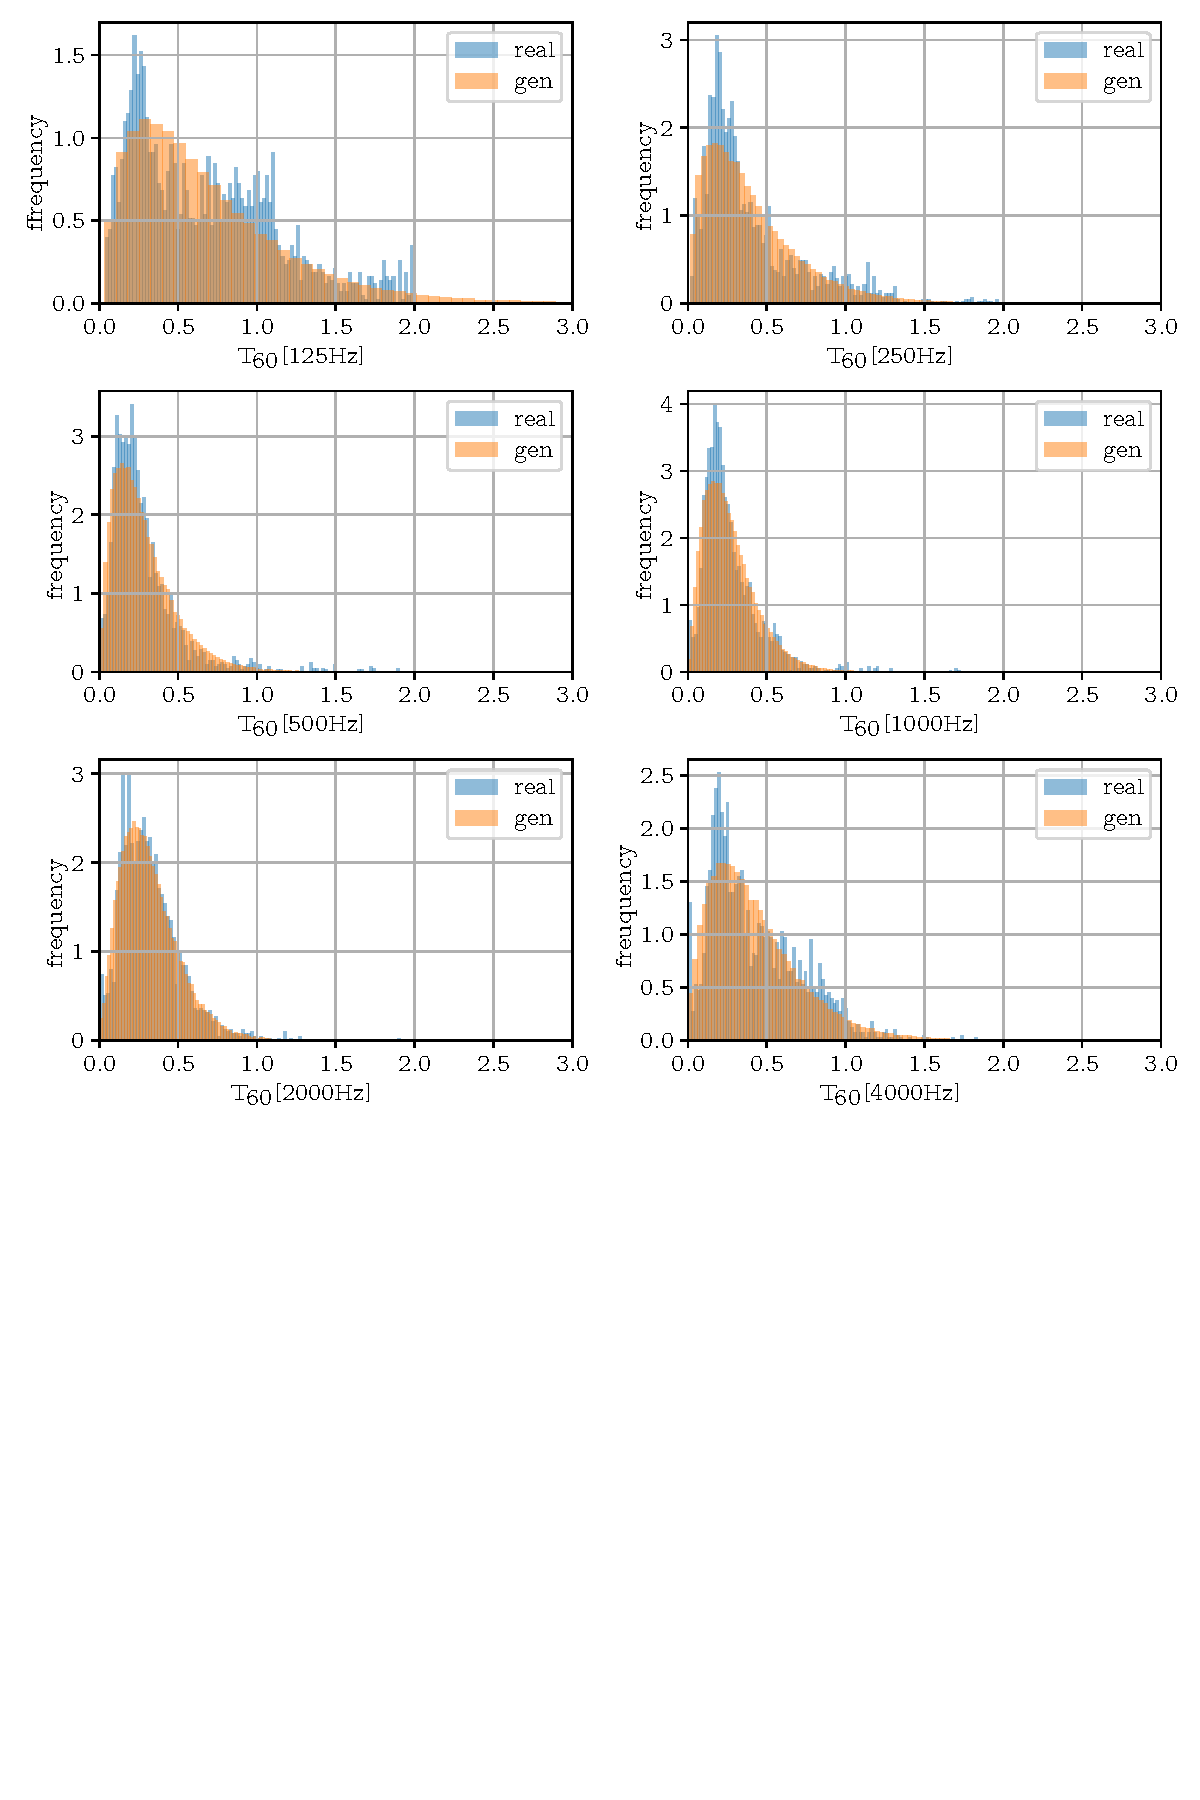
\includegraphics[width=\columnwidth,trim={0cm 11cm 0cm 0cm},clip]{ch04_mbrirs/figures/rt60Fs_sampling_distribution.pdf}
  \caption{Per-band reverberation-time distributions: the $4{.}495$ measured
  $\boldsymbol{T_{60}}$ values of \citet{sridhar2021icassp} (\emph{real}) and
  those sampled from our fitted Gamma models (\emph{gen}), for the six octave
  bands from $125\,\text{Hz}$ to $4\,\text{kHz}$. The good overall agreement in every
  band confirms that the independent per-band Gamma fits reproduce the
  statistics of real rooms.}
  \label{fig:mbrirs_t60dist}
\end{figure}


Because our \acrshort{ISM} renderer assumes a single absorption per surface, we render
one \acrshort{RIR} per band and recombine them afterwards. For each band $n$ we run an independent
\acrshort{ISM} simulation with that band's absorption, and then sum the
resulting sub-band \acrshortpl{RIR} $h_n$ after passing each through the
matching filter of an $N$-band filterbank ---a low-pass for the lowest band, a
band-pass for the intermediate ones and a high-pass for the highest:
\begin{equation}
    h \;=\; \mathrm{LPF}_{\omega_1} * h_1
      \;+\; \sum_{n=2}^{N-1} \mathrm{BPF}_{\omega_n} * h_n
      \;+\; \mathrm{HPF}_{\omega_N} * h_N .
    \label{eq:mbrirs_filterbank}
\end{equation}
The result is a single broadband \acrshort{RIR} whose decay differs across
frequency, at the cost of $N$ simulations per room instead of one.

\subsection{Receiver directivity RIRs (REC+MB)}
\label{ssec:mbrirs_rec}

The second strategy models the directivity of the \emph{receiver}. In the
\acrshort{ISM} above, both source and receiver are omnidirectional points, but
the microphones of a real capture device are not: when the device is worn on or
near the head, they inherit its acoustic shadow, so that a reflection arriving
from one side is coloured and attenuated depending on its direction of arrival.

Our motivation for modelling the head shadow directivity is that beyond its
synthetic training material, \acrshort{DNS}5 provides two special test sets of
\emph{real} noisy recordings without ground truth --- and thus evaluated only
with non-intrusive metrics --- grouped by capture device: a \emph{headset} set,
recorded with devices worn on the head such as in-ear and headset microphones,
and a \emph{speakerphone} set, recorded with hand-held or desk devices such as
laptops and mobile phones. Since our measured \acrshortpl{HRTF} approximate the
directivity of a head-worn microphone, an enhancement model trained on them should match the
acoustics of the \emph{headset} set more closely, and we would therefore expect
it to improve on that set relative to a model trained without receiver
directivity. \citet{arakawa2024quantifying} indeed found this head-and-device
directivity to be relevant for speech separation and recognition with
augmented-reality glasses.

We model it by applying a \acrshort{HRTF} to every reflection of the simulated
\acrshort{RIR}, reusing the pipeline of the hearing-aid decoder of
Chapter~\ref{ch03_hearing}. Since the \acrshortpl{RIR} produced by
\acrshort{MASP} are already expressed in the spherical-harmonic domain,
decoding them to the ear with a \acrfull{BiMagLS} decoder
\citep{engel2021improving} (Section~\ref{sec:bg_ambi_timeline}) implicitly
convolves each directional component with the corresponding \acrshort{HRTF}.
As the task is monaural, we restrict the decoding to the \emph{left} ear, using
a set of normal-hearing \acrshortpl{HRTF} of a Neumann \acrshort{KU100} dummy
head. Applied on top of the multiband set, this yields the \textbf{REC+MB}
dataset.

\subsection{Source directivity RIRs (SRC+REC+MB)}
\label{ssec:mbrirs_src}

The third strategy models the directivity of the \emph{source}. Unlike the
general case, in \acrshort{SE} the source is always speech, whose radiation is
far from omnidirectional: the human head and torso make the voice progressively
more \emph{frontal} with frequency, so that a listener behind or to the side of
the talker receives markedly less high-frequency energy. We take the average
speech radiation pattern of \citet{leishman2021high}, shown per octave band in
Figure~\ref{fig:mbrirs_srcdir}, and turn it into an azimuth--elevation lookup
table $D_{\phi,\theta}$ giving the relative radiated level in each direction and
band.

We apply this pattern \emph{within} the \acrshort{ISM}, before the final
rendering, as shown in the pipeline of Figure~\ref{fig:mbrirs_pipeline}. At that
stage the simulation has produced an \emph{echogram}: the list of reflections
reaching the receiver, each with its arrival time, amplitude and direction.
Modelling source directivity amounts to re-weighting the amplitude of every
reflection in this list by $D_{\phi,\theta}$, according to the direction in
which it \emph{left the source}. The difficulty is that the echogram stores each
reflection's direction \emph{as seen from the receiver}, not its emission angle
at the source. We recover the latter through acoustic reciprocity
\citep{samarasinghe2017acoustic}: we run a second \acrshort{ISM} simulation with
the source and receiver positions swapped, whose echogram now lists the
reflections' directions at the (original) source location. Reading the emission
angle of each reflection from this reciprocal echogram, we weight the
corresponding reflection in the original one by the matching value of
$D_{\phi,\theta}$, and only then proceed to the filterbank rendering of
Section~\ref{ssec:mbrirs_mb}. Applied on top of the receiver-directivity set,
this yields the \textbf{SRC+REC+MB} dataset.

\begin{figure}[htbp]
  \centering
  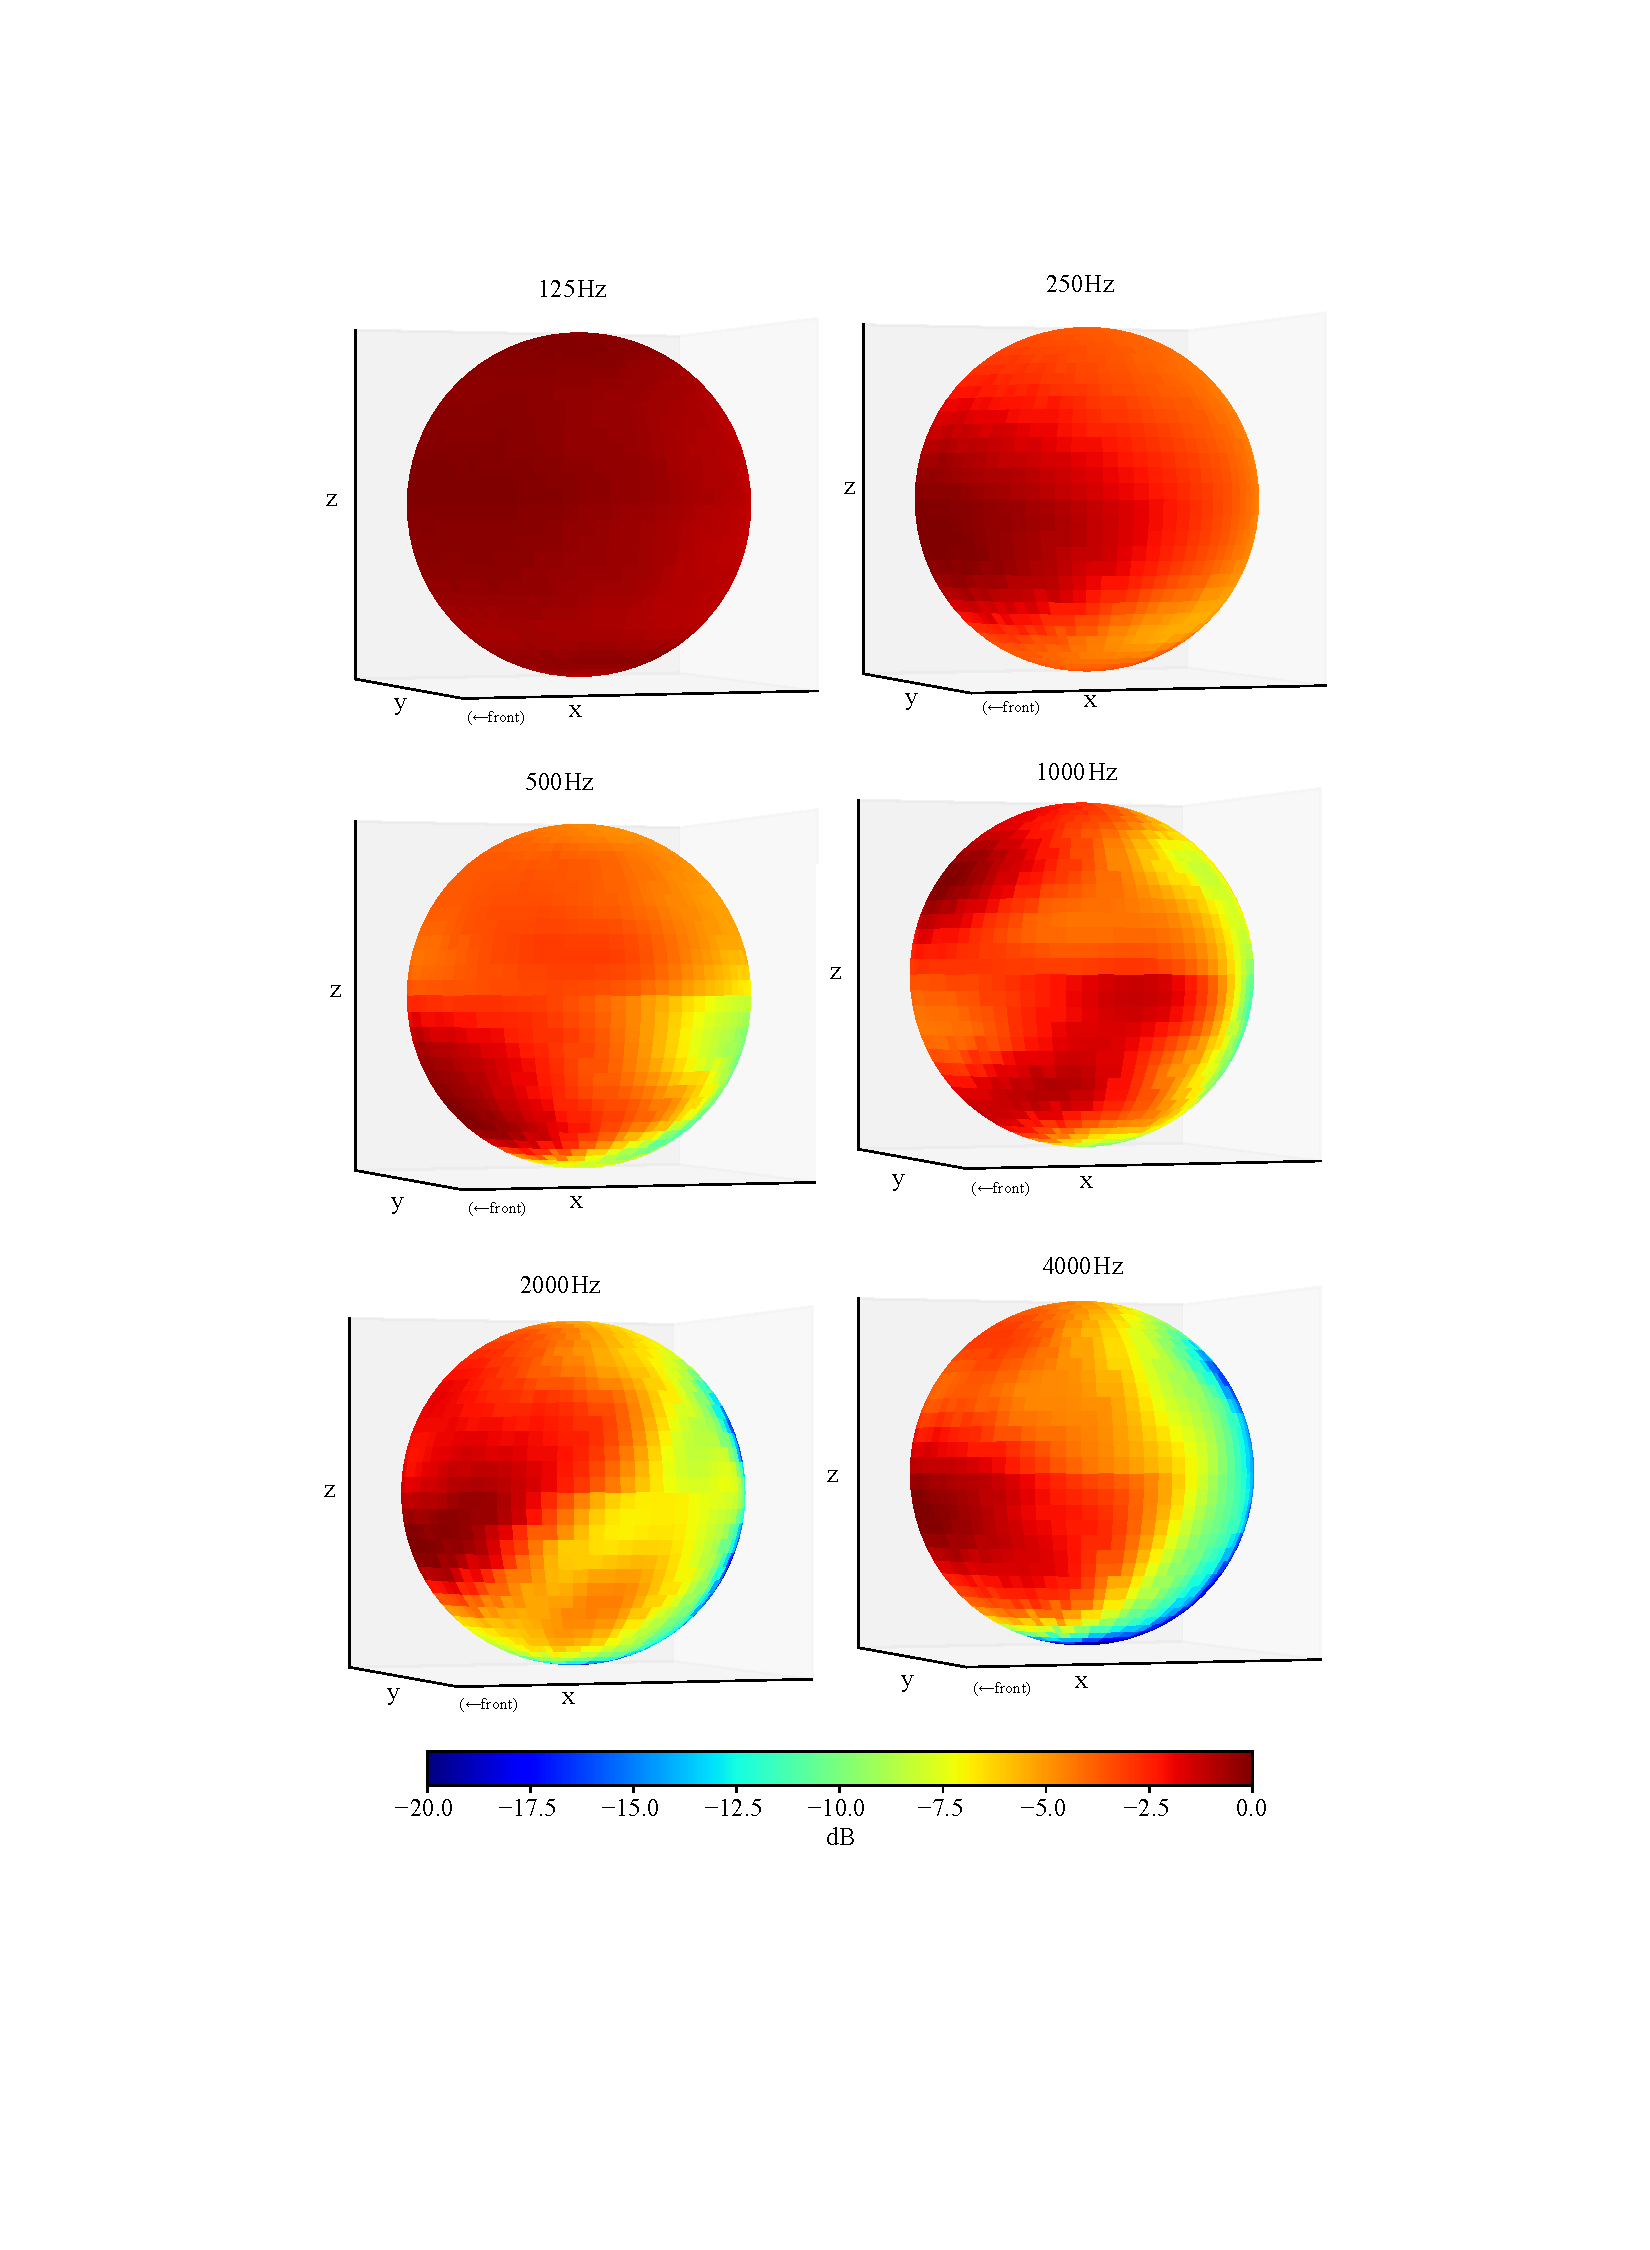
\includegraphics[width=\columnwidth,trim={5cm 6.8cm 5cm 4cm},clip]{ch04_mbrirs/figures/speech_directivity.pdf}
  \caption{Average human-speech radiation pattern $D_{\phi,\theta}$, per octave
  band from $125\,\text{Hz}$ to $4\,\text{kHz}$ \citep{leishman2021high}. Each
  sphere shows the radiated level (in dB, relative to the frontal direction
  $+x$) as a function of direction. Radiation is essentially omnidirectional at
  low frequencies and becomes increasingly frontal with frequency, the rear and
  lateral directions being attenuated by up to about $20\,\text{dB}$ at
  $4\,\text{kHz}$.}
  \label{fig:mbrirs_srcdir}
\end{figure}


\subsection{Mesh-based RIRs (SoundSpaces, SSPA)}
\label{ssec:mbrirs_sspa}

Rather than another strategy of our own, our last dataset is an external
reference: the most recent and complex synthetic \acrshort{RIR} dataset we
could find at the time, against which to contrast our \acrshort{ISM}-based
sets. It is the
one most directly comparable to our REC+MB set because it uses multi-band absorption coefficients and renders in
Ambisonics and decodes to binaural, while additionally offering the geometric realism that a shoebox
cannot. To keep the comparison fair, we take $60$k of its \acrshortpl{RIR} and,
as in REC+MB and SRC+REC+MB, use the left channel of the binaural downmix.

The crucial difference lies not in how each response is rendered, but in the
number and acoustic diversity of the rooms available: SoundSpaces spans only
$103$ scanned scenes, whereas our \acrshort{ISM}-based sets draw tens of
thousands of independent room configurations, sampling a far wider range of
sizes, geometries and per-band reverberation times. Whether the geometric
realism of a mesh outweighs this loss of acoustic coverage is precisely 
\textbf{RO4}.

\section{Experimental setup}
\label{sec:mbrirs_eval}

Given the shared speech and noise and the six \acrshort{RIR} datasets described
above, we train six \acrfull{SE} models --- one per dataset --- and evaluate
them in three complementary ways. First, we apply each model to monaural
noisy utterances convolved with \emph{real} \acrshortpl{RIR} and compute a
battery of intrusive and non-intrusive metrics
(Section~\ref{ssec:mbrirs_objective}). Second, we validate a subset of
these perceptually through a \acrfull{MUSHRA} listening test
(Section~\ref{ssec:mbrirs_res_mushra}). Third, we apply the models to the
\emph{headset} and \emph{speakerphone} test sets of \acrshort{DNS}5 to probe the
effect of receiver directivity (Section~\ref{ssec:mbrirs_res_dir}); as these contain
real mixtures without a separate clean-speech ground truth, only non-intrusive
metrics can be computed there.

As the enhancement network we use DeepFilterNet3 \citep{schroter2023deepfilternet3},
chosen because it combines state-of-the-art performance with an open-source,
real-time implementation --- the same properties that make it a plausible
candidate for deployment. All six models share its default hyperparameters,
except for a smaller maximum batch size of $38$ to fit our \acrshortpl{GPU} and
a reverberation probability $p_{\text{reverb}} = 1$, so that a \acrshort{RIR} is
applied to every utterance. Each model is trained on its own dataset for $117$
to $120$ epochs, depending on early stopping.


\subsection{Objective evaluation}
\label{ssec:mbrirs_objective}

The objective evaluation measures the \acrshort{SE} performance of each model
with a large set of metrics, over two kinds of signals, both
of which involve \emph{real} room acoustics. The first are \emph{synthetic}
mixtures, in which clean speech and noise are combined and convolved with real
\acrshortpl{RIR}; here a clean reference is available, so both intrusive and
non-intrusive metrics can be computed. The second are \emph{real recordings} (the \emph{headset} and \emph{speakerphone} sets of \acrshort{DNS}5 introduced in
Section~\ref{ssec:mbrirs_rec}) already captured as noisy mixtures in real
rooms, and therefore carrying real acoustics by construction; as they provide no
separate clean reference, only non-intrusive metrics apply. In both cases the
room acoustics are real, so the evaluation measures how well each model, trained
on \emph{synthetic} \acrshortpl{RIR}, generalises to \emph{real} ones.

For the synthetic mixtures, we take from the \acrshort{DNS}5 test split $10$k
high-quality read-speech samples --- $7$k from VCTK \citep{veaux2017cstr} and $3$k
from LibriVox \citep{panayotov2015librispeech} --- and $397$ real \acrshortpl{RIR}
gathered from the ACE \citep{eaton2015ace}, MIT IR Survey
\citep{traer2016statistics}, OpenAIR \citep{murphy2010openair} and BUT ReverbDB
\citep{szoke2019building} datasets, together with the OpenSLR28
\citep{ko2017study} responses not used in training. Each clean four-second chunk
$y$ is convolved with a real \acrshort{RIR} $h$ and mixed with a noise sample
$n$ at $\mathrm{SNR} = \mathcal{U}(0, 30)\,\text{dB}$, giving the noisy,
reverberant input $x$.

Two methodological points deserve mention. First, preserving the time alignment
between $x$ and its target $y$ proved less trivial than expected: the onset of a
\emph{real} \acrshort{RIR} is harder to detect than that of a clean synthetic
one, so rather than the widely used correlation-based synchronisation --- which
we found less robust to the noise in real responses --- we search the vicinity
of the peak amplitude for any earlier sample exceeding a $-6\,\text{dB}$
threshold, and align to that. Second, the conventional signal model
$x = (y * h) + n$ leaves the noise dry while the speech is reverberant; we
therefore also ran the whole evaluation with $x = (y + n) * h$, in which speech
and noise share a spectrally coherent reverberation at the cost of placing them
at the exact same point in space (a physically infeasible simplification). The
results were very similar, so for brevity we report only the conventional model.

The metrics we report fall into four families. \emph{Signal-fidelity} measures
compare the estimated waveform with the reference on a sample level: the
\acrfull{SI-SDR} (Section~\ref{sec:ha_metrics}) and the plain \acrfull{SDR}, in
decibels. \emph{Spectral} measures compare their time--frequency
representations: the Log-Spectral Distance (LSD) and the Mel-Frequency Cepstral Distance (MSD), both distances for
which lower is better. \emph{Perceptual} measures predict human judgements of
quality and intelligibility from an auditory model: wideband \acrfull{PESQ}
(roughly $[1, 4.5]$) and \acrfull{STOI} ($[0, 1]$). Finally, \emph{semantic}
measures, less common in \acrshort{SE}, gauge whether linguistic and speaker
content survive enhancement: a phonetic similarity, a speaker-embedding cosine
similarity, and a Bidirectional Encoder Representations from Transformers (BERT)-based textual similarity between transcripts.

Because some of these rely on a clean reference and others do not, we group them
into \emph{intrusive} metrics --- computed against the reference $y$ --- and
\emph{non-intrusive} ones, computed from the estimate alone. The latter are
increasingly estimated by neural networks trained to mimic human ratings: we
use Deep Noise Suppression Mean Opinion Score (DNSMOS, \citet{reddy2021dnsmos}) and Non-Intrusive Speech Quality Assessment (NISQA)
\citep{mittag2021nisqa}, which predict Mean Opinion Scores (MOS), and the
Speech Quality and Intelligibility Measures (SQUIM) estimators \citep{kumar2023torchaudio}, which predict
reference-free versions of \acrshort{SI-SDR}, \acrshort{PESQ}, \acrshort{STOI}
and MOS directly from the noisy signal (denoted with the subscript
$_{\text{squim}}$). Most of these follow the metric set of the URGENT challenge
\citep{zhang2024urgent}.

As in Chapter~\ref{ch03_hearing}, and because reverberation itself can bias
several of these measures, we report each metric as an \emph{increment} over the
unprocessed noisy, reverberant signal rather than as an absolute value ---
denoting it \acrshort{SI-SDR}i for the \acrshort{SI-SDR} and $\Delta m$ for the
remaining metrics $m$. For a model $f$ with estimate $\hat{y} = f(x)$,
non-intrusive metrics are computed as $m(\hat{y}) - m(x)$ and intrusive ones,
which need the reference $y$, as $m(\hat{y}, y) - m(x, y)$. On the
\emph{headset} and \emph{speakerphone} real recordings, where no clean reference
exists, only the non-intrusive metrics apply and we report their absolute
values.

For context, our evaluation deliberately reports \emph{increments} on unseen
real \acrshortpl{RIR} rather than absolute scores on a standard benchmark. On
the widely used Voicebank+Demand benchmark, DeepFilterNet reaches strong
figures: a \acrshort{PESQ} of $3.17$ and
\acrshort{STOI} of $0.944$ for the DeepFilterNet3 version we use \citep[Table~1]{schroter2023deepfilternet3}--- good results for a real-time
model, so we start from a strong baseline. Our concern here is not to improve
on those benchmarks but to test how well such a model generalises to real
room acoustics depending on the \acrshortpl{RIR} it was trained on.

\section{Results and discussion}
\label{sec:mbrirs_results}

The results confirm three findings, which we take in turn: extending the
sampling rate to $48\,\text{kHz}$ already helps; frequency-dependent absorption
(MB) brings the clearest benefit; and neither source/receiver directivity nor
mesh-based rendering brings a clear further gain, the latter being outweighed by
the smaller variety and quantity of rooms.

\subsection{Subjective results}
\label{ssec:mbrirs_res_mushra}

Figure~\ref{fig:mbrirs_mushra} shows the \acrshort{MUSHRA} scores; the means are
collected, alongside the objective metrics, in Table~\ref{tab:mbrirs_res_real}. We compare conditions with pairwise $t$-tests at a significance threshold of
$p < 0.05$. Two baselines frame the picture. First, SB significantly
outperforms the $16\,\text{kHz}$ DNS5 baseline ($p = 3\times10^{-3}$),
confirming that extending the sampling rate to $48\,\text{kHz}$ already improves
perceived quality. Second,
\acrshort{DNS}5 and SSPA are statistically indistinguishable ($p = 0.55$): despite modelling
complex geometries and furniture, and despite having the same number of
\acrshortpl{RIR} as SB, the mesh-based set spans far fewer distinct rooms,
indicating that the variety and quantity of rooms matter on top of the
complexity of each response.

\begin{figure}[htpb]
  \centering
  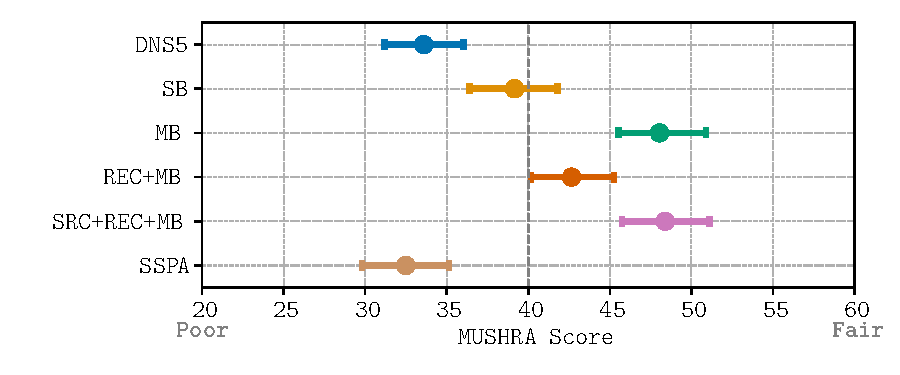
\includegraphics[trim={25 10 10 10}, clip, width=\columnwidth]{ch04_mbrirs/figures/sub_results.pdf}
  \caption{\acrshort{MUSHRA} scores (mean and $95\%$ confidence interval) for
  the six models. Higher is better.}
  \label{fig:mbrirs_mushra}
\end{figure}


Every dataset except SSPA scores significantly above the DNS5 baseline (SB:
$p = 3\times10^{-3}$; MB: $p = 7\times10^{-14}$; REC+MB: $p = 8\times10^{-7}$;
SRC+REC+MB: $p = 2\times10^{-14}$), so that both the higher sampling rate and
the added acoustic features improve enhancement. The best scores go to MB
($48.05$) and SRC+REC+MB ($48.39$), which are themselves indistinguishable
($p = 0.86$); this last equality is our first piece of evidence that modelling
directivity, while it does not help here, at least does not \emph{degrade}
monaural \acrshort{SE} on real \acrshortpl{RIR}.



\subsection{Objective results on real RIRs}
\label{ssec:mbrirs_res_obj}

\begin{table*}[t]
\centering
\scriptsize
\setlength{\tabcolsep}{2pt}
\renewcommand{\arraystretch}{1.2}
\caption{Evaluation on real \acrshortpl{RIR} with \acrshort{DNS}5 read speech
(mean $\pm$ standard deviation). Higher is better ($\uparrow$) except for LSD
and MCD ($\downarrow$). SQUIM, NISQA and DNSMOS are non-intrusive neural
estimators. Best value per row in bold.}
\label{tab:mbrirs_res_real}
\begin{tabular}{@{}llcccccc@{}}
\toprule
 & & DNS5 & SB & MB & \shortstack{REC+\\MB} & \shortstack{SRC+REC+\\MB} & SSPA \\
\midrule
\multicolumn{8}{@{}l}{\emph{Intrusive}}\\
\midrule
SI-SDRi        & $\uparrow$ & $1.105_{\pm 3.50}$ & $1.335_{\pm 3.49}$ & $1.361_{\pm 3.45}$ & $\mathbf{1.965}_{\pm 4.52}$ & $1.900_{\pm 4.41}$ & $0.888_{\pm 3.27}$ \\
$\Delta$SDR    & $\uparrow$ & $2.817_{\pm 3.17}$ & $3.298_{\pm 3.02}$ & $\mathbf{3.328}_{\pm 3.00}$ & $2.674_{\pm 3.19}$ & $2.706_{\pm 3.17}$ & $2.025_{\pm 3.11}$ \\
$\Delta$LSD    & $\downarrow$ & $1.213_{\pm 1.41}$ & $1.340_{\pm 1.42}$ & $1.260_{\pm 1.40}$ & $0.841_{\pm 1.43}$ & $\mathbf{0.778}_{\pm 1.43}$ & $1.105_{\pm 1.43}$ \\
$\Delta$MCD    & $\downarrow$ & $-1.434_{\pm 2.00}$ & $-1.479_{\pm 1.98}$ & $-1.504_{\pm 1.99}$ & $\mathbf{-1.542}_{\pm 1.97}$ & $-1.533_{\pm 1.98}$ & $-1.454_{\pm 2.00}$ \\
$\Delta$PESQ   & $\uparrow$ & $0.520_{\pm 0.47}$ & $0.583_{\pm 0.47}$ & $0.593_{\pm 0.47}$ & $0.595_{\pm 0.46}$ & $\mathbf{0.609}_{\pm 0.46}$ & $0.510_{\pm 0.45}$ \\
$\Delta$STOI   & $\uparrow$ & $0.088_{\pm 0.07}$ & $0.101_{\pm 0.07}$ & $\mathbf{0.102}_{\pm 0.07}$ & $0.101_{\pm 0.06}$ & $0.101_{\pm 0.06}$ & $0.082_{\pm 0.06}$ \\
$\Delta$PhonSim & $\uparrow$ & $0.051_{\pm 0.15}$ & $0.058_{\pm 0.15}$ & $0.058_{\pm 0.15}$ & $\mathbf{0.063}_{\pm 0.15}$ & $0.063_{\pm 0.15}$ & $0.061_{\pm 0.15}$ \\
$\Delta$SpkSim & $\uparrow$ & $-0.055_{\pm 0.13}$ & $-0.058_{\pm 0.14}$ & $-0.057_{\pm 0.13}$ & $-0.034_{\pm 0.12}$ & $\mathbf{-0.030}_{\pm 0.11}$ & $-0.053_{\pm 0.13}$ \\
$\Delta$BertSim & $\uparrow$ & $0.081_{\pm 0.07}$ & $0.086_{\pm 0.07}$ & $0.087_{\pm 0.07}$ & $0.089_{\pm 0.07}$ & $\mathbf{0.090}_{\pm 0.07}$ & $0.082_{\pm 0.07}$ \\
\midrule
\multicolumn{8}{@{}l}{\emph{Non-intrusive}}\\
\midrule
SI-SDRi$_{\text{squim}}$ & $\uparrow$ & $3.793_{\pm 5.87}$ & $4.456_{\pm 5.71}$ & $\mathbf{4.544}_{\pm 5.67}$ & $3.814_{\pm 5.65}$ & $4.038_{\pm 5.63}$ & $2.291_{\pm 5.61}$ \\
$\Delta$MOS$_{\text{squim}}$ & $\uparrow$ & $\mathbf{0.547}_{\pm 0.71}$ & $0.537_{\pm 0.71}$ & $0.541_{\pm 0.71}$ & $0.523_{\pm 0.70}$ & $0.506_{\pm 0.71}$ & $0.541_{\pm 0.70}$ \\
$\Delta$MOS$_{\text{dnsmos}}$ & $\uparrow$ & $0.884_{\pm 0.53}$ & $0.935_{\pm 0.54}$ & $\mathbf{0.937}_{\pm 0.53}$ & $0.895_{\pm 0.53}$ & $0.906_{\pm 0.53}$ & $0.811_{\pm 0.52}$ \\
$\Delta$MOS$_{\text{nisqa}}$ & $\uparrow$ & $1.158_{\pm 0.73}$ & $1.198_{\pm 0.73}$ & $\mathbf{1.224}_{\pm 0.72}$ & $1.109_{\pm 0.72}$ & $1.099_{\pm 0.72}$ & $0.977_{\pm 0.73}$ \\
$\Delta$PESQ$_{\text{squim}}$ & $\uparrow$ & $0.636_{\pm 0.62}$ & $0.667_{\pm 0.59}$ & $\mathbf{0.678}_{\pm 0.59}$ & $0.613_{\pm 0.58}$ & $0.637_{\pm 0.58}$ & $0.525_{\pm 0.57}$ \\
$\Delta$STOI$_{\text{squim}}$ & $\uparrow$ & $0.060_{\pm 0.08}$ & $0.070_{\pm 0.08}$ & $\mathbf{0.071}_{\pm 0.08}$ & $0.063_{\pm 0.08}$ & $0.066_{\pm 0.08}$ & $0.048_{\pm 0.08}$ \\
\midrule
\multicolumn{8}{@{}l}{\emph{Subjective}}\\
\midrule
MUSHRA & $\uparrow$ & $33.59_{\pm 20.3}$ & $39.15_{\pm 22.6}$ & $48.05_{\pm 22.8}$ & $42.65_{\pm 22.5}$ & $\mathbf{48.39}_{\pm 23.0}$ & $32.49_{\pm 21.7}$ \\
\bottomrule
\end{tabular}
\end{table*}



The objective metrics on the same real-\acrshort{RIR} test set, in
Table~\ref{tab:mbrirs_res_real}, broadly echo the listening test: MB
\acrshortpl{RIR} tend to outperform the rest. There is, however, no full
consensus. Most intrusive metrics favour MB and SRC+REC+MB, in line with the
subjective scores, but \acrshort{SI-SDR}, MCD and phonetic similarity instead
point to REC+MB. The non-intrusive metrics agree more closely, with MB
slightly ahead ($p < 0.05$) --- possibly a bias of the NISQA and SQUIM
predictors, though, interestingly, one that favours MB rather than the simpler
SB. Overall, the multiband sets behave very similarly to one another and clearly
above DNS5 and SSPA, so the objective and subjective evidence agree on the main
point: multiband absorption is the change that brings the clearest benefit,
with MB and SRC+REC+MB at the top and indistinguishable from one another.

\subsection{Directivity and the device-specific sets}
\label{ssec:mbrirs_res_dir}

The \emph{headset} and \emph{speakerphone} sets were meant to isolate the effect
of directivity, under the hypothesis that receiver-directivity models
(REC+MB, SRC+REC+MB) should match the head-worn \emph{headset} recordings more
closely.

\begin{table}[t]
\centering
\footnotesize
\setlength{\tabcolsep}{4pt}
\renewcommand{\arraystretch}{1.2}
\caption{Non-intrusive evaluation on the real \acrshort{DNS}5 \emph{headset}
(HDS) and \emph{speakerphone} (SPK) recordings. Higher is better; best per row
in bold.}
\label{tab:mbrirs_res_spk}
\begin{tabular}{@{}llcccccc@{}}
\toprule
 & & DNS5 & SB & MB & REC+MB & SRC+REC+MB & SSPA \\
\midrule
\multirow{2}{*}{SI-SDR$_{\text{squim}}$} & HDS & $15.65$ & $15.75$ & $\mathbf{15.80}$ & $15.35$ & $15.42$ & $14.21$ \\
                                         & SPK & $16.81$ & $16.86$ & $\mathbf{17.05}$ & $16.65$ & $16.82$ & $15.51$ \\[2pt]
\multirow{2}{*}{MOS$_{\text{squim}}$}    & HDS & $3.92$ & $3.89$ & $3.90$ & $3.91$ & $\mathbf{3.94}$ & $3.91$ \\
                                         & SPK & $\mathbf{4.15}$ & $\mathbf{4.15}$ & $\mathbf{4.15}$ & $4.14$ & $4.14$ & $4.14$ \\[2pt]
\multirow{2}{*}{MOS$_{\text{dnsmos}}$}   & HDS & $3.01$ & $3.04$ & $\mathbf{3.05}$ & $3.04$ & $3.02$ & $3.01$ \\
                                         & SPK & $3.03$ & $3.05$ & $\mathbf{3.06}$ & $3.03$ & $3.04$ & $2.99$ \\[2pt]
\multirow{2}{*}{MOS$_{\text{nisqa}}$}    & HDS & $3.54$ & $3.64$ & $\mathbf{3.68}$ & $3.61$ & $3.56$ & $3.43$ \\
                                         & SPK & $3.77$ & $3.82$ & $\mathbf{3.82}$ & $3.77$ & $3.76$ & $3.62$ \\[2pt]
\multirow{2}{*}{PESQ$_{\text{squim}}$}   & HDS & $2.58$ & $2.59$ & $\mathbf{2.62}$ & $2.55$ & $2.54$ & $2.45$ \\
                                         & SPK & $2.64$ & $2.63$ & $\mathbf{2.64}$ & $2.56$ & $2.59$ & $2.49$ \\[2pt]
\multirow{2}{*}{STOI$_{\text{squim}}$}   & HDS & $0.92$ & $0.92$ & $0.92$ & $0.92$ & $0.92$ & $0.91$ \\
                                         & SPK & $0.94$ & $0.94$ & $0.94$ & $0.94$ & $0.94$ & $0.93$ \\
\bottomrule
\end{tabular}
\end{table}

Table~\ref{tab:mbrirs_res_spk} shows this hypothesis is not borne out.
On both sets, most non-intrusive metrics again put the MB models marginally
ahead, as on the real-\acrshort{RIR} test, but the differences are not
statistically significant (e.g.\ $p = 0.9$ for $\text{SI-SDR}_{\text{squim}}$
between MB and SB), and REC+MB and SRC+REC+MB show no advantage on the
\emph{headset} set. We therefore find no evidence of a benefit from directivity
modelling.

Although \citet{arakawa2024quantifying} showed that directivity can be exploited
even by monaural models, we could not reproduce that effect --- whether because
of the limitations of the NISQA and SQUIM predictors or of the \acrshort{DNS}5
device sets themselves. This leaves open a question we cannot settle here: do MB
\acrshortpl{RIR} help because they are more \emph{domain-consistent} with real
rooms, or simply because they are more \emph{diverse} than SB \citep{jeon2024does}?
Directivity does not degrade performance and may yet help, but on this evidence
we cannot claim a clear improvement.

\subsection{Summary}
\label{ssec:mbrirs_res_summary}

Taken together, the results recommend training \acrshort{SE} models on varied,
high-sampling-rate multiband \acrshortpl{RIR}, optionally adding source and
receiver directivity depending on the use case. This answers \textbf{RO3} in the
affirmative for frequency-dependent absorption --- which benefits modern
\acrshort{SE} as it had benefited keyword spotting --- and more cautiously for
directivity, which does no harm but shows no clear gain. It answers \textbf{RO4}
in the negative: geometric realism does not, on its own, compensate for a loss of
room diversity, as the amount and variety of \acrshortpl{RIR} prove as important
as the complexity of each one. We release the two most useful sets, MB and
SRC+REC+MB, as the \emph{MB-RIRs}
dataset.

\section{Conclusions}
\label{sec:mbrirs_conclusions}

This chapter has asked which properties of a synthetic \acrshort{RIR} improve
the \emph{ecological validity} of the training data --- and thereby the
generalisation of monaural \acrshort{SE} models to real room acoustics --- and
has answered it by training a state-of-the-art, real-time model
(DeepFilterNet3) on six \acrshort{RIR} datasets that differ in a single,
controlled feature at a time.

Regarding \textbf{RO3}, extending the \acrshortpl{RIR} with
frequency-dependent absorption coefficients --- an idea previously shown to help
keyword spotting --- also benefits modern \acrshort{SE}, and is the change that
brings the clearest and most consistent improvement across objective and
subjective evaluation. Extending the sampling rate from $16$ to $48\,\text{kHz}$
already helps on its own. Source and receiver directivity, by contrast, neither
degrade performance nor yield a clear gain: they may help, but on our evidence
we cannot claim a definite improvement, and the hypothesis that receiver
directivity would benefit the head-worn \emph{headset} recordings was not borne
out.

Regarding \textbf{RO4}, geometric realism does not, on its own, compensate for a
smaller variety and quantity of rooms: the mesh-based SoundSpaces set, despite
modelling complex geometries, did not outperform the far more numerous
\acrshort{ISM} shoebox rooms, and was statistically indistinguishable from the
baseline. The amount and variability of the \acrshortpl{RIR} thus prove as
important as the complexity of each individual response: for the ecological
validity of a \acrshort{RIR} dataset, \emph{coverage} of the space of real rooms
weighs as heavily as the physical fidelity of any single response --- a theme
that runs through this thesis.

One limitation of this answer to \textbf{RO4} is that the mesh-based condition
confounds two factors: SoundSpaces is at once geometrically realistic and
limited to few rooms, so its poor performance cannot be attributed to the
mesh-based rendering alone. Disentangling them would require a mesh-based
dataset that also offers a large acoustic variety, such as GWA
\citep{tang2022gwa}, which renders millions of responses over tens of thousands
of rooms with a hybrid wave-based and ray-tracing simulator
(Chapter~\ref{ch02_sota}). Repeating our evaluation with GWA in place of
SoundSpaces would test whether mesh-based rendering helps once the loss of room
variety is removed; we leave this comparison for future work.

In conclusion, improving the ecological validity of the training
\acrshortpl{RIR} measurably improves \acrshort{SE} generalisation to real
rooms. We recommend training on varied, $48\,\text{kHz}$ multiband
\acrshortpl{RIR}, optionally adding source and receiver directivity depending on
the use case, and we release the two most useful datasets, MB and SRC+REC+MB, as
\emph{MB-RIRs}, freely available as research
material.\footnote{\url{https://doi.org/10.5281/zenodo.15773093}}
